

\tikzset{every picture/.style={line width=0.75pt}} %set default line width to 0.75pt

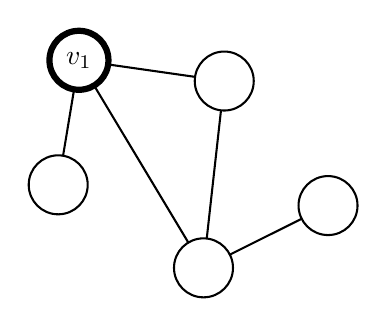
\begin{tikzpicture}[x=0.75pt,y=0.75pt,yscale=-1,xscale=1]
%uncomment if require: \path (0,169); %set diagram left start at 0, and has height of 169


% Text Node
\draw  [line width=2.25]   (45, 32) circle [x radius= 14.21, y radius= 14.21]   ;
\draw (45,32) node   [align=left] {\begin{minipage}[lt]{13.600000000000001pt}\setlength\topsep{0pt}
\begin{center}
$\displaystyle v_{1}$
\end{center}

\end{minipage}};
% Text Node
\draw    (115, 42) circle [x radius= 14.21, y radius= 14.21]   ;
\draw (115,42) node   [align=left] {\begin{minipage}[lt]{13.600000000000001pt}\setlength\topsep{0pt}
\begin{center}
$ $
\end{center}

\end{minipage}};
% Text Node
\draw    (35, 92) circle [x radius= 14.21, y radius= 14.21]   ;
\draw (35,92) node   [align=left] {\begin{minipage}[lt]{13.600000000000001pt}\setlength\topsep{0pt}
\begin{center}
$ $
\end{center}

\end{minipage}};
% Text Node
\draw    (105, 132) circle [x radius= 14.21, y radius= 14.21]   ;
\draw (105,132) node   [align=left] {\begin{minipage}[lt]{13.600000000000001pt}\setlength\topsep{0pt}
\begin{center}
\end{center}

\end{minipage}};
% Text Node
\draw    (165, 102) circle [x radius= 14.21, y radius= 14.21]   ;
\draw (165,102) node   [align=left] {\begin{minipage}[lt]{13.600000000000001pt}\setlength\topsep{0pt}
\begin{center}
$ $
\end{center}

\end{minipage}};
% Connection
\draw    (42.66,46.02) -- (37.34,77.98) ;
% Connection
\draw    (59.07,34.01) -- (100.93,39.99) ;
% Connection
\draw    (52.31,44.19) -- (97.69,119.81) ;
% Connection
\draw    (113.43,56.13) -- (106.57,117.87) ;
% Connection
\draw    (117.71,125.64) -- (152.29,108.36) ;

\end{tikzpicture}